%  !TeX spellcheck = en_GB
%  WangSheying于2015/11/2整理,TJU北洋园校区
%  TeXLive2015+TeXstudio个人推荐,可在线升级usepackage,比较方便
%*****************************************************************************************
%  从这里开始到\begin{document}是导言区,称之为preamble
\documentclass[UTF8]{beamer}
\usepackage[fontset=mac]{ctex}
%\usepackage[UTF8]{ctex}                 %使用中文要添加,可解决中文文档输入
\usepackage{newtxtext,newtxmath}  %字重齐全的高质量数学字体
\usepackage{mathrsfs}             %大写ABC的花体使用命令是\mathscr{}
\usepackage{graphicx}             %添加图片
\usepackage{bm}                   %专门处理数学粗体的bm宏包,使用命令是\bm{}
\usepackage{extarrows}            %延长符号,可在=,->等符号加多个字母
%\usepackage{amstext}              %它定义命令 \text,可用于在数学公式中插入少量文本,并可调整上下标中文本字体的尺寸。
\usepackage{amsthm}               %它定义了一个 proof 环境,用来排版定理和证明,能自动在最后添加证毕符号。它还提供一个命令:\newtheorem{定理环境名}{标题}[计数器名],可自定义定理类 环境
\usefonttheme{professionalfonts}  %这个更好看些,数学字体
\usepackage{indentfirst}          %首行缩进
\usepackage{verbatim}
\usepackage{amsmath}
\usepackage{amsfonts}
\usepackage{amssymb}
\usepackage{xcolor}
\usepackage{subfigure}
\usepackage[english]{babel}
\usepackage{algorithm}
\usepackage{algorithmic}
\usepackage{tikz}
\setlength{\parindent}{2em}      %首行缩进2字符
\setbeamertemplate{theorems}[numbered]
\setbeamertemplate{caption}[numbered]
%******************************************************************************************
%            以上是各种宏包
%******************************************************************************************
%下面是定理,定义,引言的声明,可自行添加

\newtheorem{thm}{Theorem}
\newtheorem{lem}[thm]{Lemma}
\newtheorem{cor}[thm]{Corollary}
\newtheorem{prop}[thm]{Proposition}
\newtheorem{defi}[thm]{Definition}
\newtheorem{remark}[thm]{Remark}
\newtheorem{claim}[thm]{Claim}

\newenvironment{proofnoqed}{\begin{proof}<span style="background-color: rgb(255, 0, 0);">\renewcommand{\qedsymbol}{}  }{\end{proof} }
%有的证明比较长,前面的应该没有证毕符号,只在最后一个用proof,其他应该用自定义的新环境proofnoqed



%  三种颜色   red  purple   magenta





%上面是定理,定义,引言的声明,可自行添加
%******************************************************************************************
%下面是beamer的主题设置,目录框架结构,其实就是标题,目录等在上下左右哪一个位置放置,以及目录怎么显示
\usetheme{Singapore}            % 幻灯片模板选择singapore
\usecolortheme{sidebartab}      % 幻灯片模板的色彩sidebartab

\AtBeginSection[]{              % 幻灯片框架% 在每个Section前都会加入的Frame,
	\begin{frame}[plain]
		\frametitle{Outline}
		\tableofcontents[sectionstyle=show/shaded,subsectionstyle=show/show/shaded]
	\end{frame} 
}
%  \tableofcontents[comma-separated option list]具体讲解见《The beamer class User Guide》,
%  http://texdoc.net/texmf-dist/doc/latex/beamer/doc/beameruserguide.pdf     See in section 10.5 Adding a table of contents.
%  section和subsection相互独立,显示效果互不相关,Allowed ⟨styles⟩ are show, shaded, and hide
%  sectionstyle=⟨style for current section⟩/⟨style for other sections⟩
%  subsectionstyle=⟨style for current subsection⟩/⟨style for other subsections in current section⟩/⟨style for subsections in other sections⟩
%
% 上面是beamer的主题设置,目录框架结构,其实就是标题,目录等在上下左右哪一个位置放置,以及目录怎么显示
%*******************************************************************************************
%       下面标题页的内容设置,根据实际情况修改即可
\title{深入理解Kafka: 核心设计与实现原理}  % 幻灯片封面
\author{王社英}
\institute{北京回龙观}
\date{\today}  

%\date{9月 23, 2019}%一般是\today
%      上面标题页的内容设置根据实际情况修改即可
%*******************************************************************************************
%  \begin{document}以上是导言区,称之为preamble
%*******************************************************************************************
\begin{document}
	\begin{frame}[plain]
		%plain格式使得一帧的最上面是白色的,没有plain,会有色彩
		\titlepage
	\end{frame}
	\begin{frame}[plain]               % 幻灯片目录
		\frametitle{Outline}
		\tableofcontents[sectionstyle=show/show,subsectionstyle=show/show/hide]
	\end{frame}
	%The beamer class这本小册子有目录格式的讲解,sectionstyle,subsectionstyle都有,P100页
	%User Guide for version 3.36. 文档可在google搜索The beamer class,即可得到
%  以上是标准的配置,还有最下面的一部分标准配置
%********************************************************************************************
%    一帧的具体格式样例参考
%\section{节的名字}
%\subsection{小节的名字}
%\begin{frame}[plain,t]{节的名字} %也可以使用\frametitle{节的名字}效果一样
%	\structure{小节的名字} \\  \vspace{2ex}
%	节的名字正上方居中,小节的名字紧下方居左。
%\end{frame}
%*********************************************************************************************
%                  下面就是正文,自己的内容
%*********************************************************************************************

\section{初识Kafka}
\begin{frame}[plain,t]{Kafka简介} %也可以使用\frametitle{节的名字}效果一样
	%\structure{} \\
	  \vspace{2ex}
	Kafka定位为一个分布式流式处理平台,具有以下特性:
	\begin{itemize}
		\item 高吞吐
		\item 可持久化
		\item 可水平扩展
		\item 支持流数据处理
	\end{itemize}
	\vspace{2ex}
	
	Kafka扮演的三大角色
	\begin{enumerate}
		\item 消息系统
		\item 存储系统
		\item 流式处理平台
	\end{enumerate}
	

	
	
\end{frame}
\subsection{ 基本概念}
\begin{frame}[plain,t]{基本概念} %也可以使用\frametitle{节的名字}效果一样
	\structure{体系架构} \\  
	\vspace{2ex}
	\begin{figure}
		\centering
		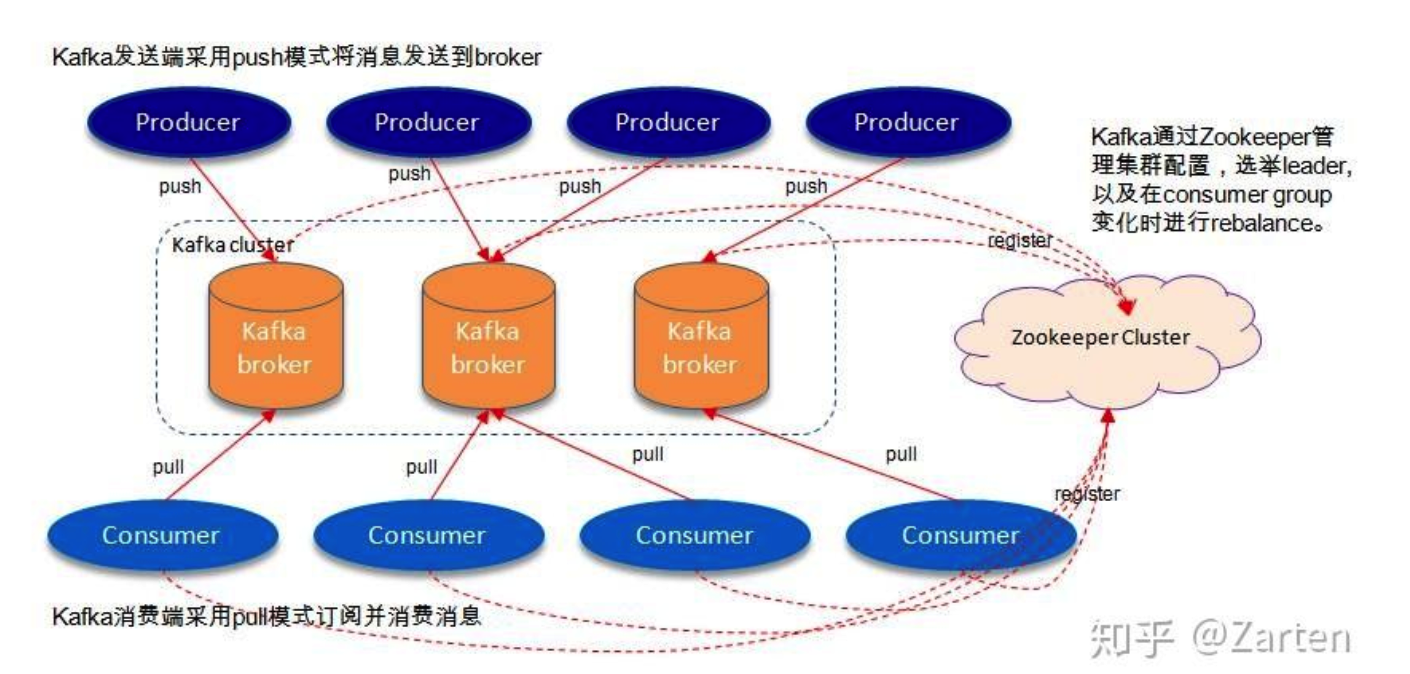
\includegraphics[width=0.9\linewidth]{image/0101}
		\caption{kafka体系架构图}
		\label{fig:0101}
	\end{figure}
	
     
\end{frame}
\begin{frame}[plain,t]{基本概念} %也可以使用\frametitle{节的名字}效果一样
	\structure{体系架构} \\  
	 \vspace{2ex}
	 	\begin{figure}
	 	\centering
	 	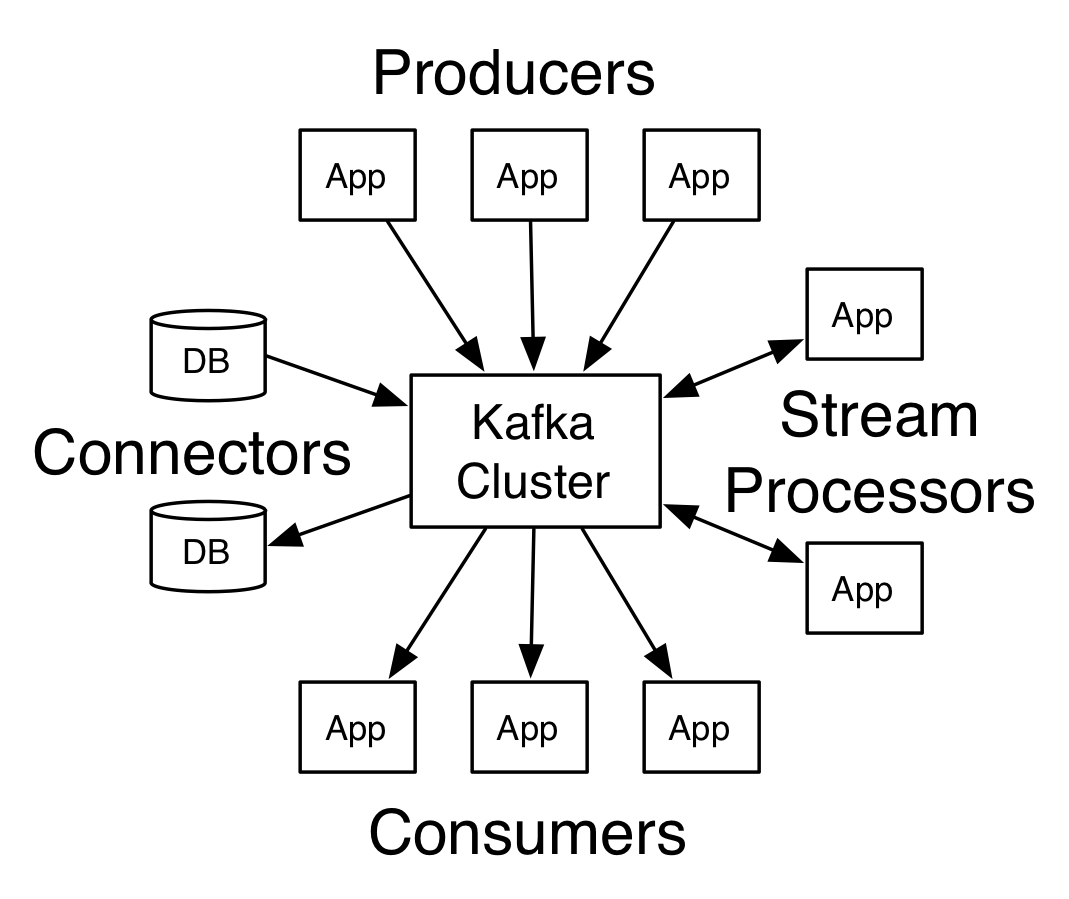
\includegraphics[width=0.7\linewidth]{image/0102}
	 	\caption{kafka体系架构图}
	 	\label{fig:0102}
	 \end{figure}
	
	
	
\end{frame}
\begin{frame}[plain,t]{基本概念} %也可以使用\frametitle{节的名字}效果一样
\structure{体系架构} \\  
	 \vspace{2ex}
	 整个Kafka体系结构分3部分:
	 \begin{itemize}
	 	\item Producer
	 	\item Consumer
	 	\item Broker
	 \end{itemize}
 
 \vspace{2ex}
 Kafka的三层消息架构:
 \begin{itemize}
 	\item Topic
 	\item Partition
 	\item Record
 \end{itemize}
 
 
	
	
	
\end{frame}
\begin{frame}[plain,t]{基本概念} %也可以使用\frametitle{节的名字}效果一样
	\structure{体系架构} \\  
	 \vspace{2ex}
	 \begin{figure}
	 	\centering
	 	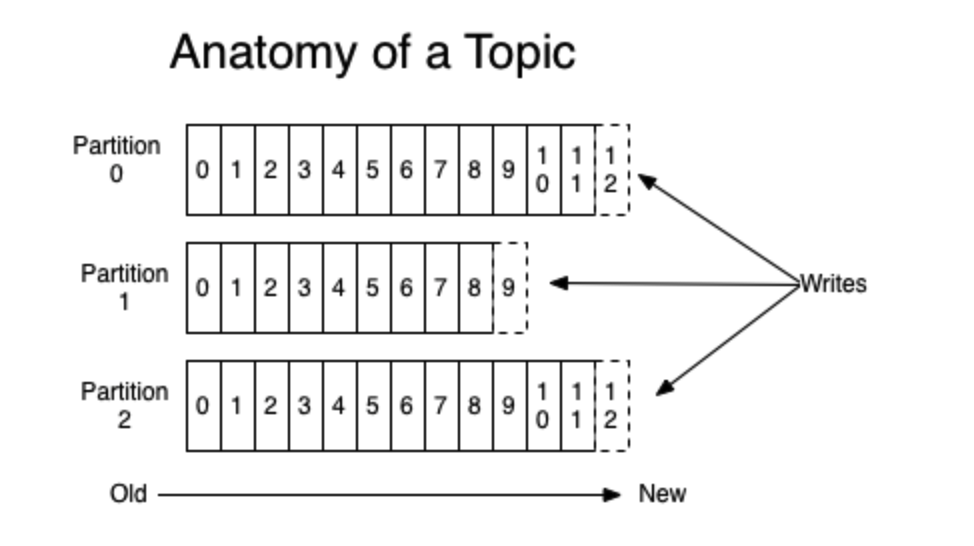
\includegraphics[width=0.9\linewidth]{image/0103}
	 	\caption{消息追加--分区视角}
	 	\label{fig:0103}
	 \end{figure}
	 
\end{frame}
\begin{frame}[plain,t]{基本概念} %也可以使用\frametitle{节的名字}效果一样
		\structure{体系架构} \\  
	\vspace{2ex}
	\begin{figure}
		\centering
		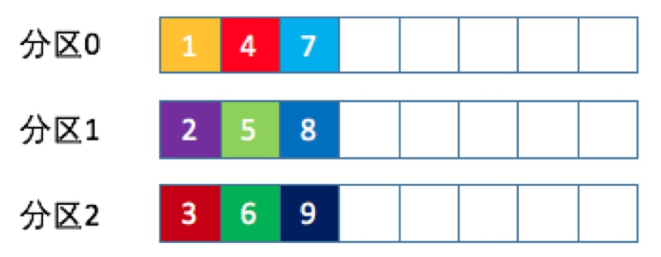
\includegraphics[width=0.9\linewidth]{image/0104}
		\caption{消息追加--生产者视角}
		\label{fig:0104}
	\end{figure}
	
	
\end{frame}

\begin{frame}[plain,t]{基本概念} %也可以使用\frametitle{节的名字}效果一样
		\structure{高可用} \\  
	 \vspace{2ex}
	 Kafka高可用机制:
	 \begin{itemize}
	 	\item AR(Assigned Replicas)
	 	\item ISR(In-Sync Replicas)
	 	\item OSR(Out-of-Sync Replicas)
	 \end{itemize}
 \vspace{2ex}
 
 在正常情况下,所有的follower副本都应该与leader副本保持一定程度的同步
 AR=ISR,OSR=$\varnothing$
 
 \begin{figure}
 	\centering
 	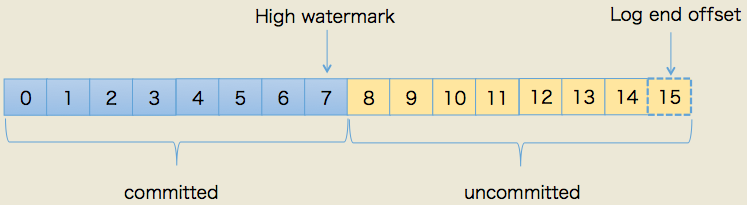
\includegraphics[width=0.9\linewidth]{image/0105}
 	\caption{HW和LEO}
 	\label{fig:0105}
 \end{figure}
 
	
\end{frame}
\begin{frame}[plain,t]{基本概念} %也可以使用\frametitle{节的名字}效果一样
\structure{数据一致性} \\  
	\vspace{1ex}

	 \begin{figure}
		\centering
		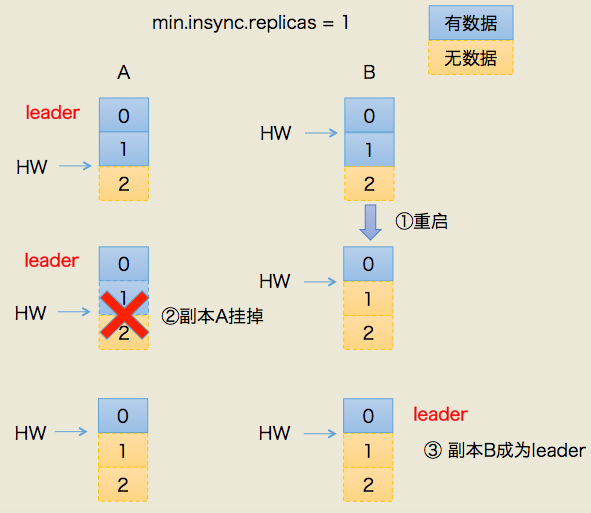
\includegraphics[width=0.75\linewidth]{image/0106}
		\caption{数据丢失}
		\label{fig:0106}
	\end{figure}
	
\end{frame}
\begin{frame}[plain,t]{基本概念} %也可以使用\frametitle{节的名字}效果一样
\structure{数据一致性} \\  
	\vspace{1ex}

	\begin{figure}
		\centering
		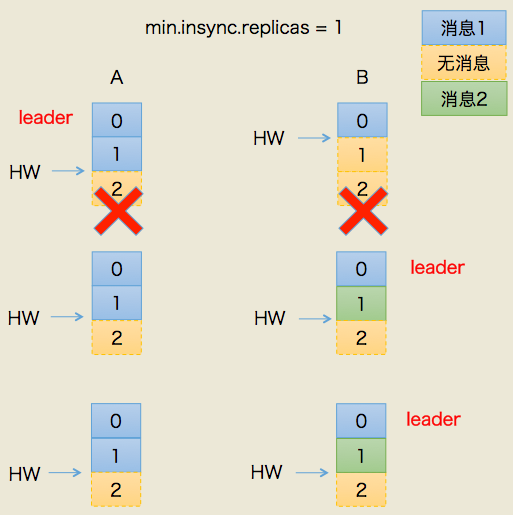
\includegraphics[width=0.6\linewidth]{image/0107}
		\caption{数据不一致}
		\label{fig:0107}
	\end{figure}
	
	
	
\end{frame}
\begin{frame}[plain,t]{基本概念} %也可以使用\frametitle{节的名字}效果一样
\structure{数据一致性} \\  \vspace{2ex}
	\begin{figure}
		\centering
		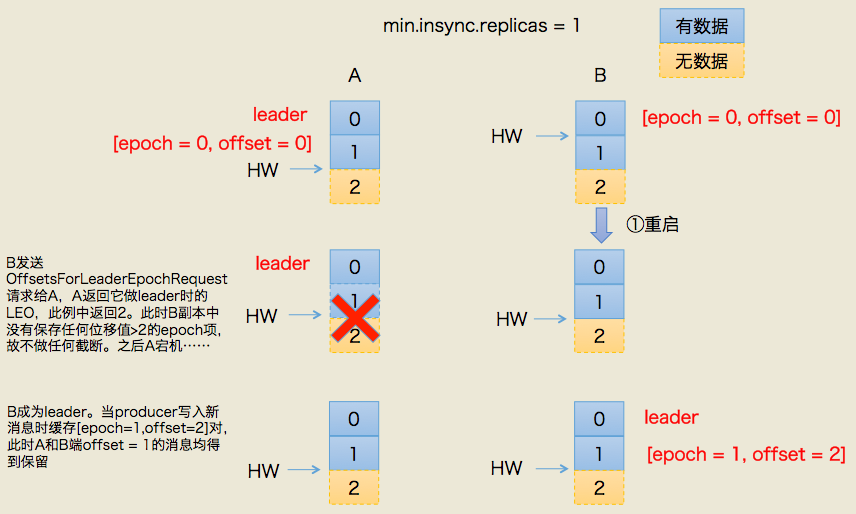
\includegraphics[width=0.9\linewidth]{image/0108}
		\caption{leader epoch规避数据丢失}
		\label{fig:0108}
	\end{figure}
	
\end{frame}
\begin{frame}[plain,t]{基本概念} %也可以使用\frametitle{节的名字}效果一样
\structure{数据一致性} \\  \vspace{1ex}

	\begin{figure}
		\centering
		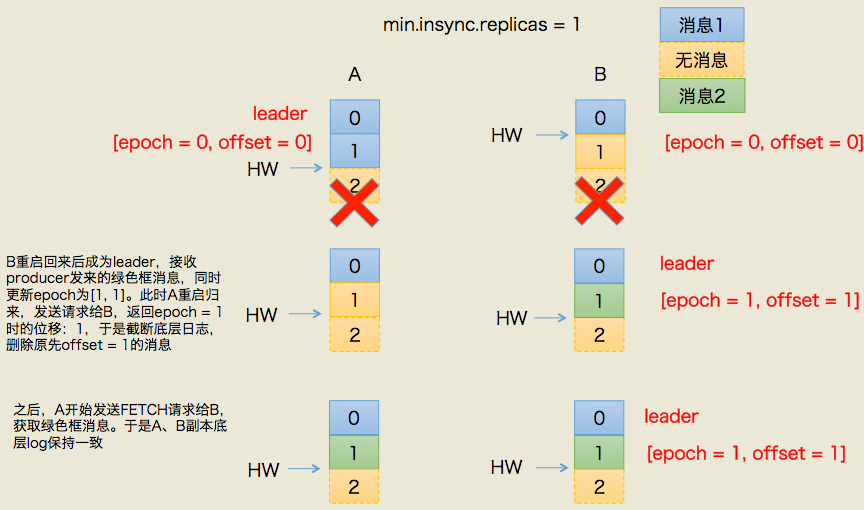
\includegraphics[width=0.9\linewidth]{image/0109}
		\caption{leader epoch规避数据不一致}
		\label{fig:0108}
	\end{figure}
	
\end{frame}


\section{生产者}
\subsection{原理分析}
\begin{frame}[plain,t]{原理分析} %也可以使用\frametitle{节的名字}效果一样
	\structure{消息的发送} \\ 
	 \vspace{2ex}
	KafkaProducer是线程安全的,可以在多个线程中共享单个KafkaProducer实例,也可以将KafkaProducer实例进行池化
	来供其他线程调用.
	
	 \vspace{1ex}
	 生产者发送消息的三种模式:
	 \begin{itemize}
	 	\item fire-and-forget
	 	\item sync
	 	\item async
	 \end{itemize}
 
 KafkaProducer.send()返回值是Future<RecordMetadata>.
 
 Future表示一个任务的生命周期,提供了相应的方法判断
  \begin{itemize}
 	\item 任务状态,完成或取消
 	\item 任务结果
 	\item 取消任务
 \end{itemize}

\end{frame}
\begin{frame}[plain,t]{原理分析} %也可以使用\frametitle{节的名字}效果一样
\structure{消息的发送} \\  \vspace{2ex}
	 生产者发送消息常见异常:
	  \vspace{1ex}
	 \begin{itemize}
	 	\item 可重试异常
	 	 \begin{itemize}
	 		\item NetworkException,
	 		\item LeaderNotAvailableException
	 		\item UnknownTopicOrPartitionException
	 		\item NotEnoughReplicasException
	 		\item NotCoordinatorException
	 	\end{itemize}
	 	\item 不可重试异常
	 	 \begin{itemize}
	 		\item RecordTooLargeException
	 	\end{itemize}
	 \end{itemize}
 
 
	 
	

\end{frame}
\begin{frame}[plain,t]{原理分析} %也可以使用\frametitle{节的名字}效果一样
	\structure{消息的发送} \\  \vspace{2ex}
	生产者需要用序列化器(Serializer)把对象转换成字节数组才能通过网络发送给Kafka.
	\vspace{2ex}
	
	消息在通过send()方法发往broker的过程中,有可能需要经过拦截器(Interceptor,{\color{red} 可选}),序列化器(Serializer,{\color{cyan}必选})和分区器(Partitioner,{\color{brown}默认轮询})
	的一系列作用之后才能被真正发往broker.
	
\end{frame}
\begin{frame}[plain,t]{原理分析} %也可以使用\frametitle{节的名字}效果一样
	\structure{整体架构} \\  \vspace{2ex}
	\begin{figure}
		\centering
		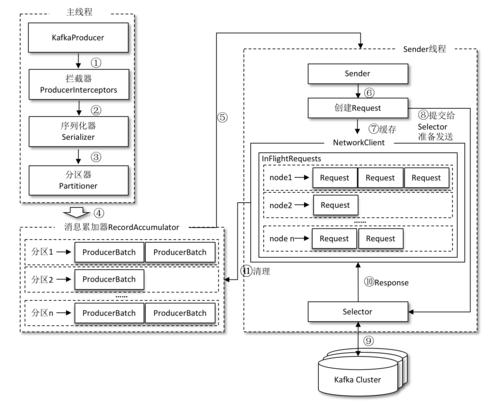
\includegraphics[width=0.7\linewidth]{image/0201}
		\caption{生产者客户端整体架构}
		\label{fig:0201}
	\end{figure}
	
\end{frame}
\begin{frame}[plain,t]{原理分析} %也可以使用\frametitle{节的名字}效果一样
	\structure{整体架构} \\  \vspace{2ex}
		
		\begin{center}
			ProducerRecord \\
			$\Downarrow$ \\
			ProducerBatch \\
			$\Downarrow$ \\
			 <Partition, Deque<ProducerBatch> > \\
			 $\Downarrow$ \\
			 <Node, List<ProducerBatch> > \\
			 $\Downarrow$ \\
			 <Node, Request> \\
			 $\Downarrow$ \\
			 Broker
		\end{center}
	
\end{frame}
\begin{frame}[plain,t]{原理分析} %也可以使用\frametitle{节的名字}效果一样
	\structure{整体架构} \\  \vspace{2ex}
	元数据是指Kafka集群的元数据,这些元数据具体记录了集群中有哪些Topic,这些Topic有哪些Partition,
	每个Partition的leader副本分配在哪个Broker上,follower副本分配在哪些Broker上,哪些副本在AR,ISR集合中,
	集群有哪些Broker,控制器Broker又是哪一个等信息.
	 \vspace{2ex}
	 
	 当客户端中没有这些元数据信息时,或者超过metadata.max.age.ms(默认5分钟)时,都会更新元数据.
	 \vspace{2ex}
	 
	 元数据的更新是由Sender线程负责的,主线程也需要读取这些信息,数据同步通过synchronized和final关键字来保障.
\end{frame}



\section{消费者}
\subsection{Kafka Consuming Model}
\begin{frame}[plain,t]{Kafka Consuming Model} %也可以使用\frametitle{节的名字}效果一样
	\structure{消费者与消费者组} \\  \vspace{2ex}
	
	同一个分片只能由消费者分组中的同一个消费者进行消费

	\begin{figure}
		\centering
		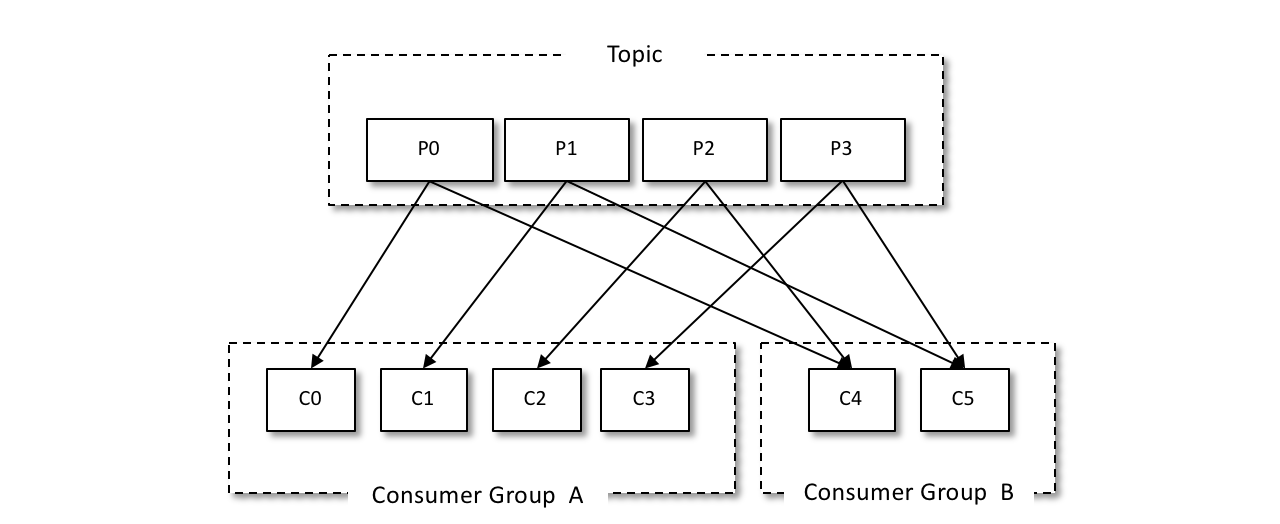
\includegraphics[width=0.9\linewidth]{image/0301}
		%\caption{}
		\label{fig:0301}
	\end{figure}
	
\end{frame}
\begin{frame}[plain,t]{Kafka Consuming Model} %也可以使用\frametitle{节的名字}效果一样
	\structure{消费者与消费者组} \\ 
	\begin{figure}
		\centering
		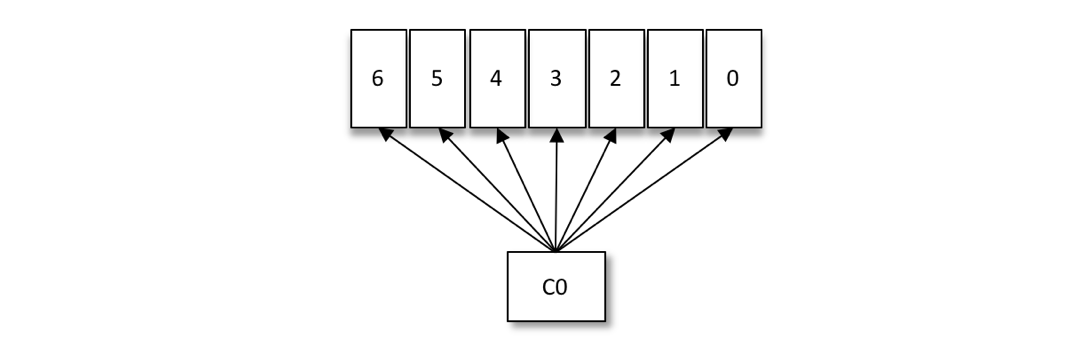
\includegraphics[width=0.9\linewidth]{image/0302}
		%\caption{}
		\label{fig:0302}
	\end{figure}
 \vspace{-4ex}
	\begin{figure}
		\centering
		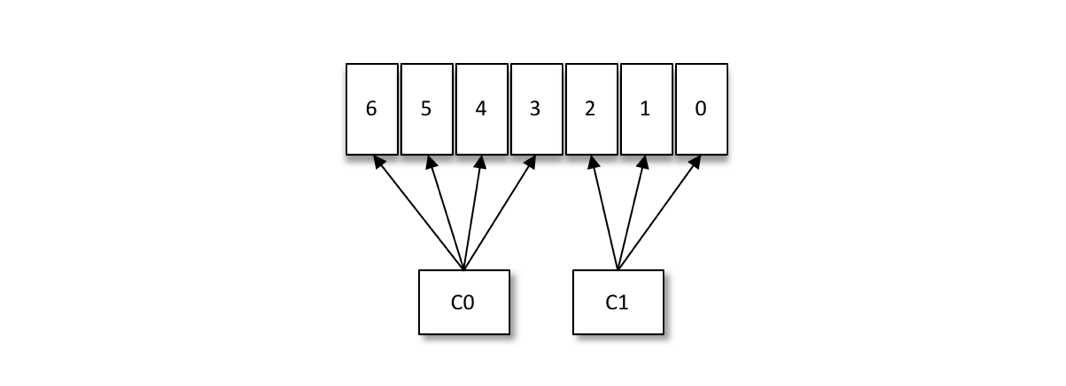
\includegraphics[width=0.9\linewidth]{image/0303}
		%\caption{}
		\label{fig:0303}
	\end{figure}
\end{frame}
\begin{frame}[plain,t]{Kafka Consuming Model} %也可以使用\frametitle{节的名字}效果一样
	\structure{消费者与消费者组} \\ 
	\begin{figure}
		\centering
		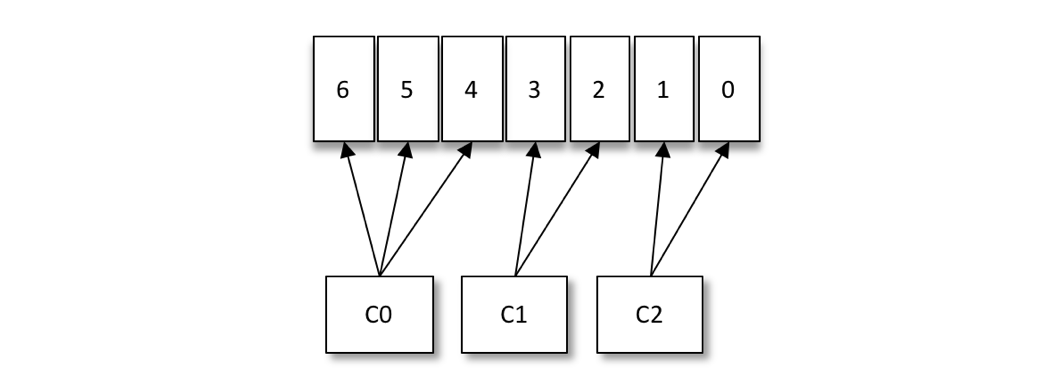
\includegraphics[width=0.9\linewidth]{image/0304}
		%\caption{}
		\label{fig:0304}
	\end{figure}
 \vspace{-4ex}
\begin{figure}
	\centering
	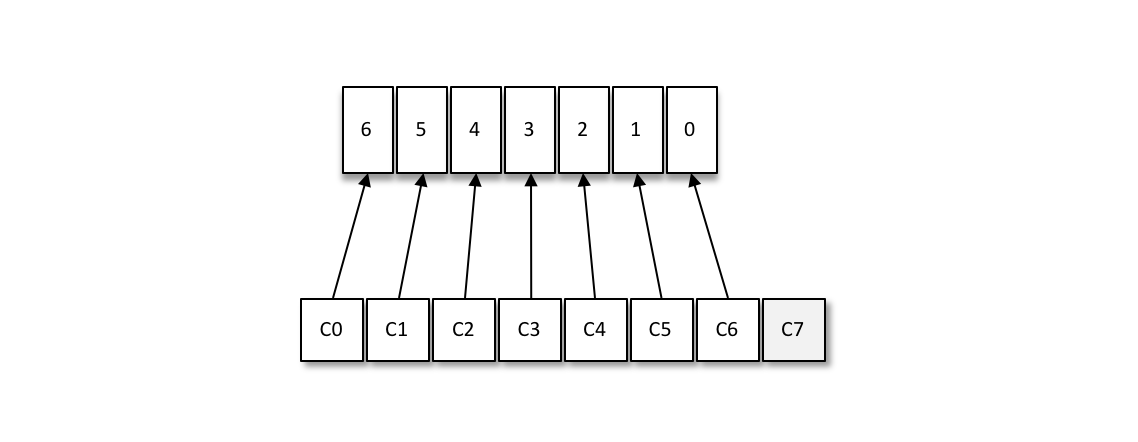
\includegraphics[width=0.9\linewidth]{image/0305}
	%\caption{}
	\label{fig:0305}
\end{figure}

	
\end{frame}



\begin{frame}[plain,t]{Kafka Consuming Model} %也可以使用\frametitle{节的名字}效果一样
	\structure{消息消费} \\  \vspace{2ex}
	Kafka中的消费是基于pull模式,消费者主动向服务器发起请求拉取消息.
	
	\vspace{2ex}
	Kafka中的消息消费是一个不断轮询的过程,消费者重复调用poll()方法.
	
		\vspace{2ex}
		poll()方法返回的是所订阅主题(分区)上的一组消息,如果没有可供消费的消息,则返回空集.
	
\end{frame}
\begin{frame}[plain,t]{Kafka Consuming Model} %也可以使用\frametitle{节的名字}效果一样
	\structure{Consumer启动时消费位移} \\  \vspace{2ex}
	
	\begin{figure}
		\centering
		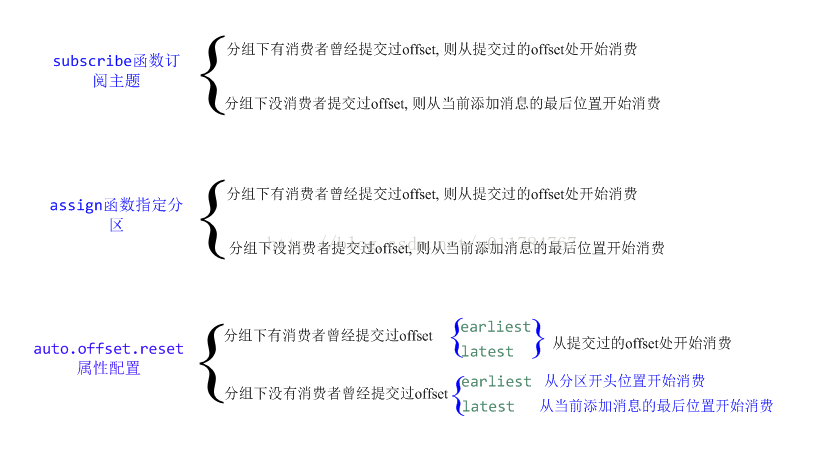
\includegraphics[width=0.9\linewidth]{image/0312}
		\caption{Consumer启动时消费位移}
		\label{fig:0312}
	\end{figure}
	
\end{frame}
\begin{frame}[plain,t]{Kafka Consuming Model} %也可以使用\frametitle{节的名字}效果一样
	\structure{Consumer启动时消费位移} \\  \vspace{2ex}
	\begin{figure}
		\centering
		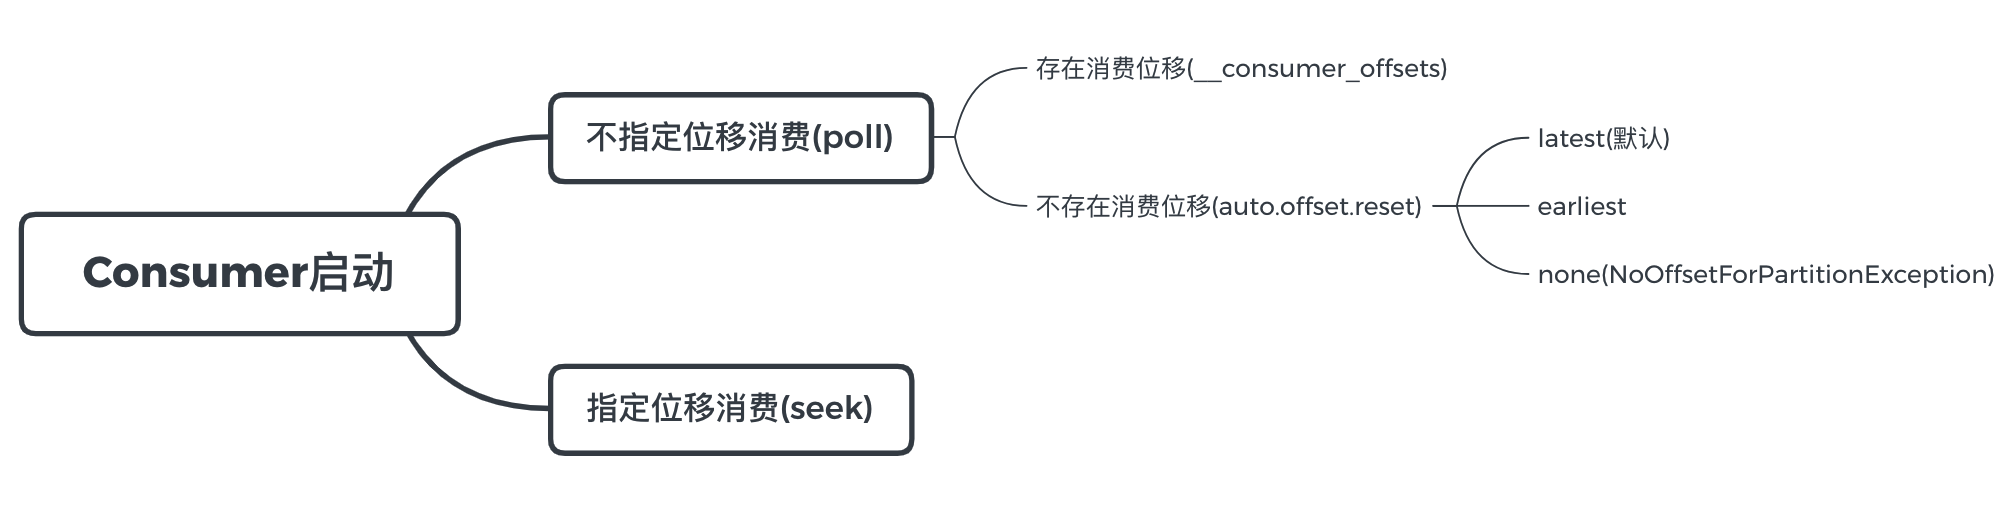
\includegraphics[width=1\linewidth]{image/0313}
		\caption{Consumer启动时消费位移}
		\label{fig:0313}
	\end{figure}
	
\end{frame}
\begin{frame}[plain,t]{Kafka Consuming Model} %也可以使用\frametitle{节的名字}效果一样
	\structure{位移提交服务端} \\  \vspace{2ex}
	
	It has never changed from a external point of view, but internally, it did since Kafka 0.9, and the appearance of the {\color{red}\_\_consumer\_offsets}. 
	
	\vspace{2ex}
A Group Coordinator is an Offset Manager(GroupMetadataManager) at the same time. It’s a broker which is the leader for a group, that caches and commits its consumers offsets.
	
		\vspace{2ex}
	It’s saved as binary data, each message in this topic has a key({\color{red}group, topic, partition number}) and a value.
	
	\begin{figure}
		\centering
		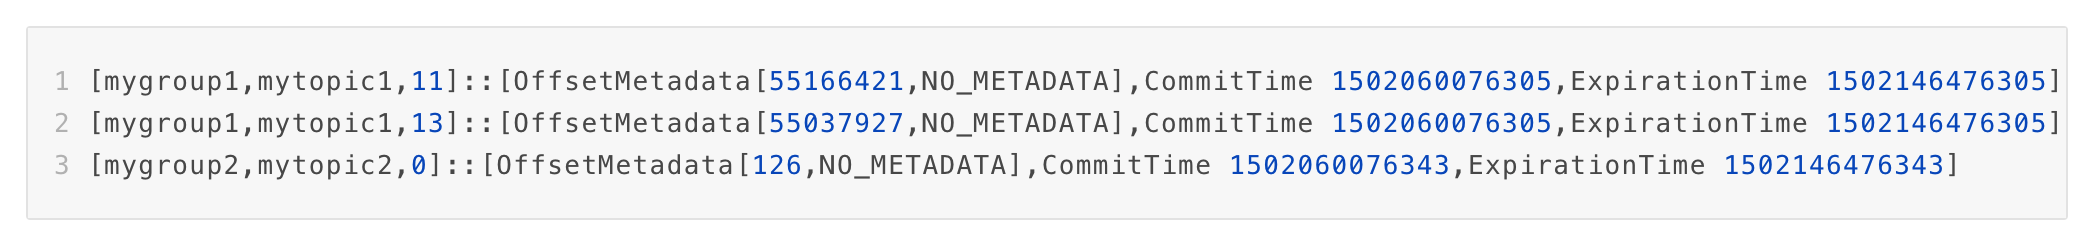
\includegraphics[width=1\linewidth]{image/0308}
		\caption{\_\_consumer\_offsets key:value}
		\label{fig:0308}
	\end{figure}
	
	


\end{frame}

\begin{frame}[plain,t]{Kafka Consuming Model} %也可以使用\frametitle{节的名字}效果一样
	\structure{位移提交服务端} \\  \vspace{2ex}
	\begin{figure}
		\centering
		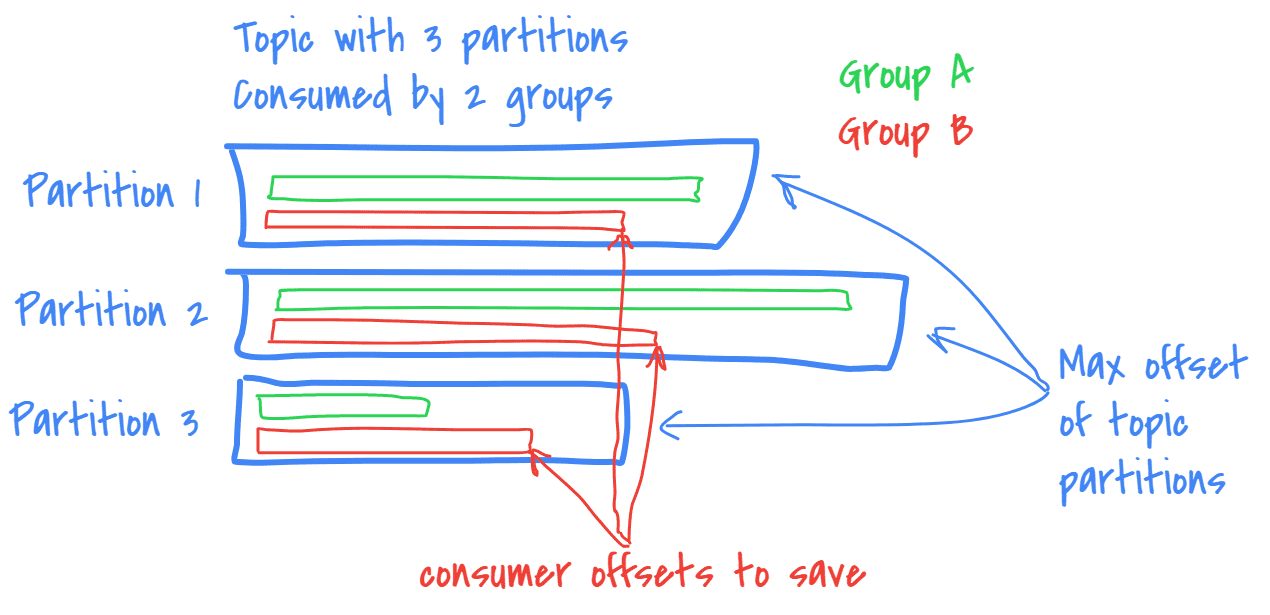
\includegraphics[width=0.9\linewidth]{image/0306}
		%\caption{(partition,topic,groupId)}
		\label{fig:0306}
	\end{figure}
	
\end{frame}
\begin{frame}[plain,t]{Kafka Consuming Model} %也可以使用\frametitle{节的名字}效果一样
	\structure{位移提交服务端} \\  \vspace{2ex}
	
	\begin{figure}
		\centering
		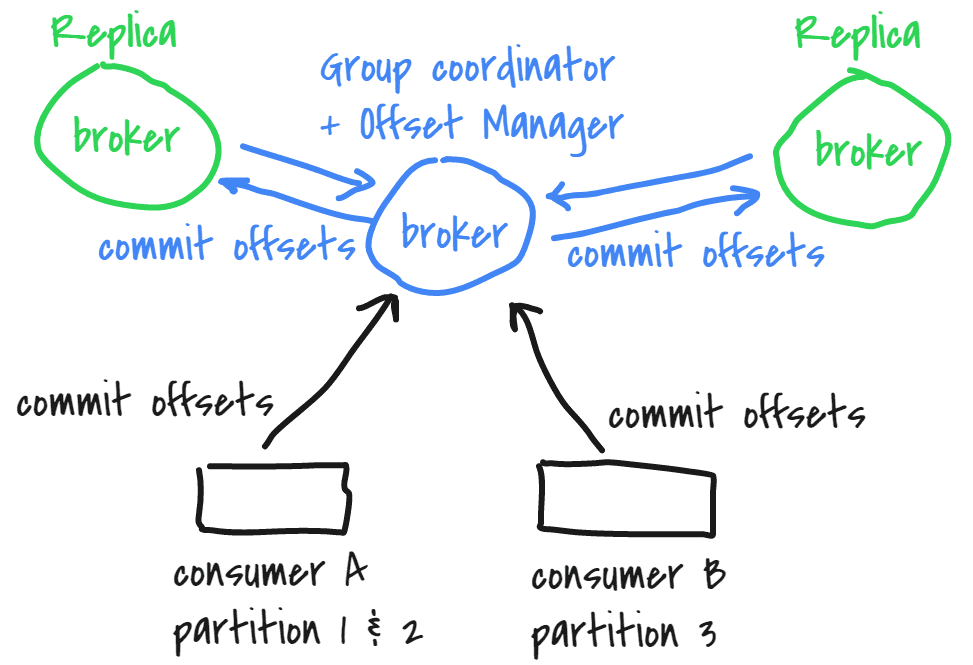
\includegraphics[width=0.85\linewidth]{image/0309}
		%\caption{(partition,topic,groupId)}
		\label{fig:0309}
	\end{figure}
	
\end{frame}
\begin{frame}[plain,t]{Kafka Consuming Model} %也可以使用\frametitle{节的名字}效果一样
	\structure{位移提交服务端} \\  \vspace{2ex}
	\begin{figure}
		\centering
		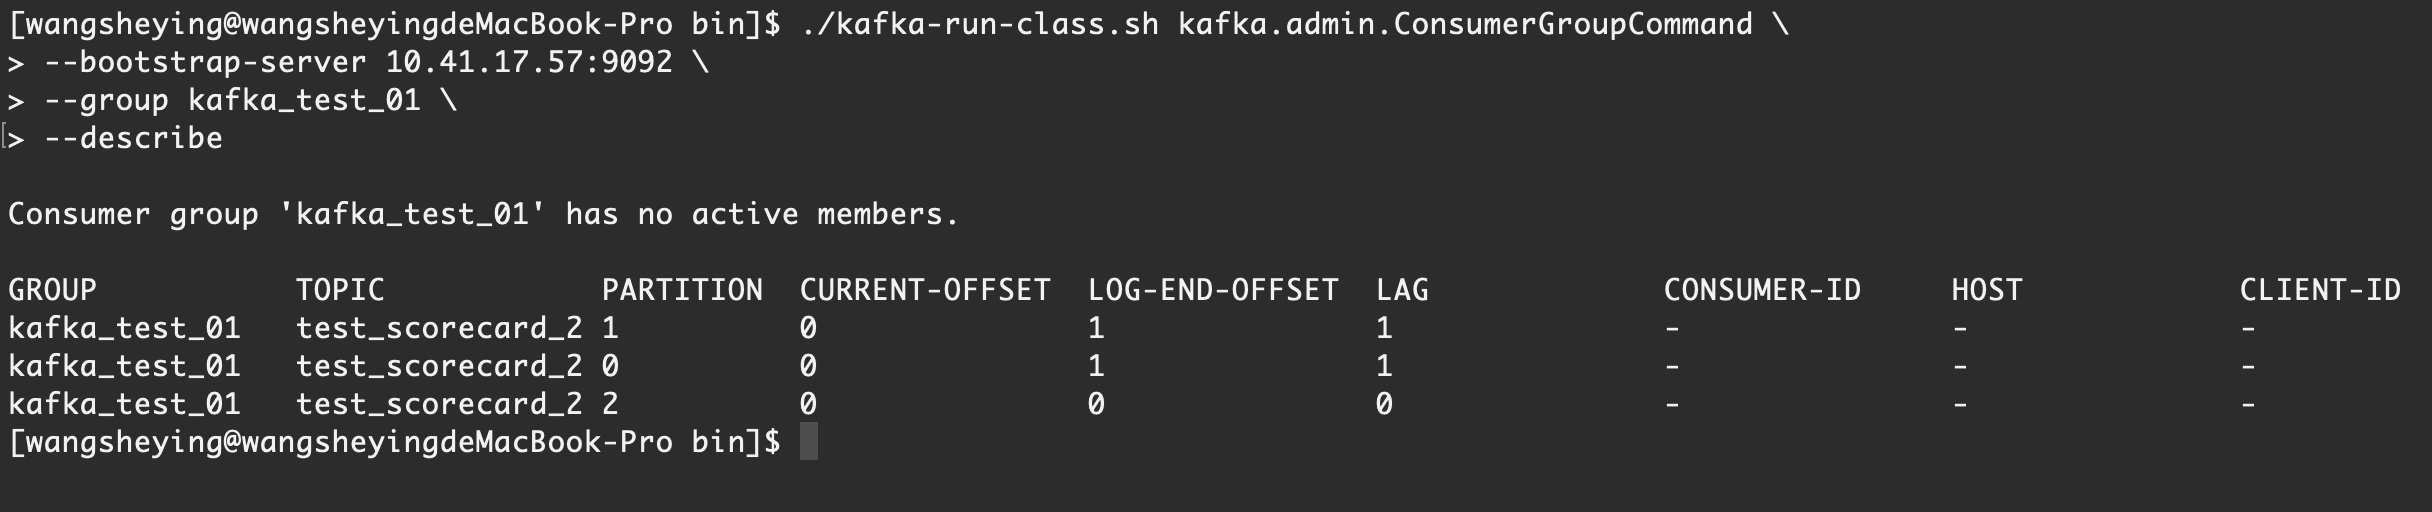
\includegraphics[width=0.95\linewidth]{image/0307}
		\caption{kafka-run-class.sh kafka.admin.ConsumerGroupCommand}
		\label{fig:0307}
	\end{figure}
	
\end{frame}


\begin{frame}[plain,t]{Kafka Consuming Model} %也可以使用\frametitle{节的名字}效果一样
	\structure{位移提交服务端} \\  \vspace{2ex}
	Conclusion
	\begin{itemize}
		\item \_\_consumer\_offsets is an implementation detail (came in 0.9) we should not rely on; it replaces the old system based on Zookeeper.
		\item \_\_consumer\_offsets is binary encoded. It keeps the latest consumed offsets for each topic/group/partition for a certain time only (1d, 过期自动删除).
		\item ConsumerGroupCommand can be used to retrieve the consumers offsets.
		\item There is one broker that deals with offset commits: the GroupCoordinator/OffsetManager.
		\item Low-level consumers can choose to not commit their offsets into Kafka (mostly to ensure at-least/exactly-once).
	\end{itemize}
\end{frame}
\begin{frame}[plain,t]{Kafka Consuming Model} %也可以使用\frametitle{节的名字}效果一样
	\structure{位移提交客户端} \\  \vspace{2ex}
	位移提交是 Kafka 提供的一个语义保障,即如果你提交了位移 X,那么 Kafka 会认为所有位移值{\color{cyan}小于 X} 的消息你都已经成功消费了。
	
	\vspace{2ex}
	位移提交的语义保障需要由{\color{red} Comsumer}来负责,Kafka 只会“无脑”地接受提交的位移
	
	
	\begin{itemize}
		\item 自动提交
		\begin{itemize}
			\item enable.auto.commit (默认true)
			\item auto.commit.interval.ms (默认5s)
		\end{itemize}
		\item 手动提交
		\begin{itemize}
			\item 同步提交
			\item 异步提交
		\end{itemize}
	\end{itemize}
\end{frame}

\begin{frame}[plain,t]{Kafka Consuming Model} %也可以使用\frametitle{节的名字}效果一样
	\structure{自动提交特性} \\  \vspace{2ex}
	Kafka 保证在开始调用 poll 方法时,提交上次 poll 返回的所有消息. 
	
	\vspace{2ex}
	从顺序上来说,poll 方法的逻辑是先提交上一批消息的位移,再处理下一批消息.
	\begin{itemize}
		\item 保证不丢失
		\item 可能会重复
	\end{itemize}

\vspace{2ex}
但是存在缓存池的情况下,可能丢失.


\end{frame}

\begin{frame}[plain,t]{Kafka Consuming Model} %也可以使用\frametitle{节的名字}效果一样
	\structure{手动提交特性} \\  \vspace{2ex}
	\begin{itemize}
		\item 同步提交 
		\begin{itemize}
			\item 阻塞
			\item 自动重试
		\end{itemize}
		\item 异步提交
		\begin{itemize}
			\item 不阻塞
			\item 不会重试(位移值可能早已“过期”或不是最新值)
		\end{itemize}
	\end{itemize}
\end{frame}

\begin{frame}[plain,t]{Kafka Consuming Model} %也可以使用\frametitle{节的名字}效果一样
	\structure{手动提交特性} \\  \vspace{2ex}
	确保关闭消费者或再均衡前的最后一次提交成功
	\begin{figure}
		\centering
		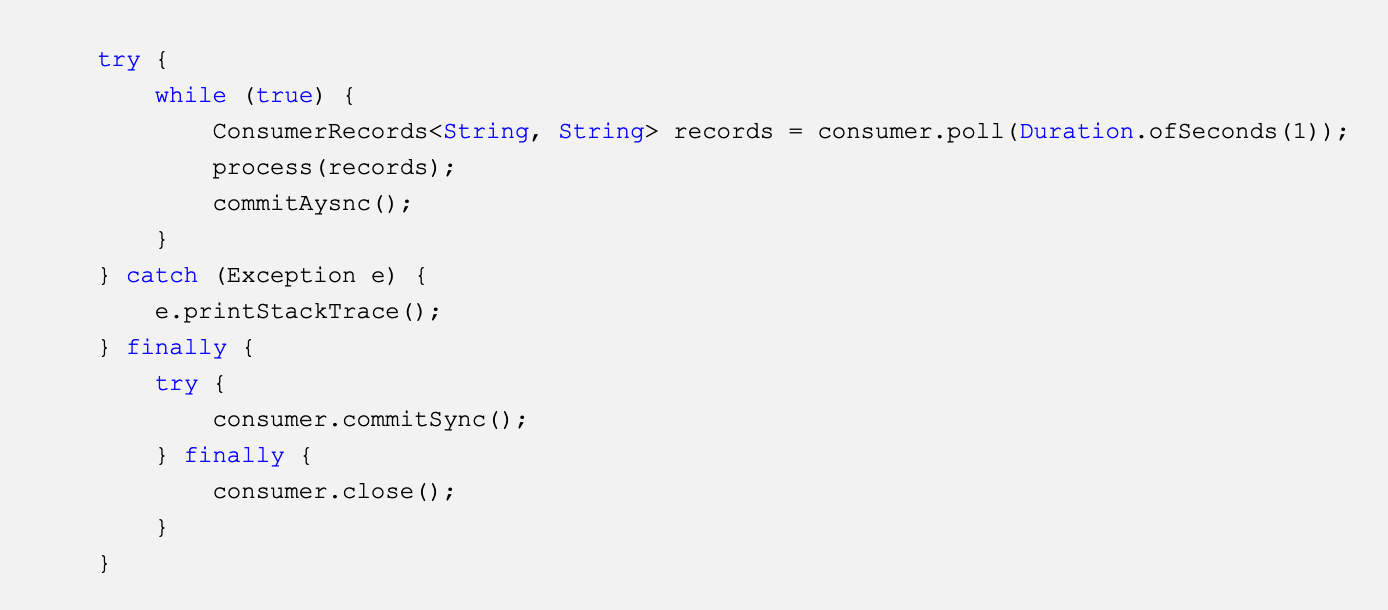
\includegraphics[width=0.9\linewidth]{image/0310}
		\caption{同步异步组合提交}
		\label{fig:0310}
	\end{figure}
	
\end{frame}
\begin{frame}[plain,t]{Kafka Consuming Model} %也可以使用\frametitle{节的名字}效果一样
	\structure{手动提交特性} \\  \vspace{2ex}
	如果一次拉取了很多消息但是没有消费完,提交已经消费完成的位置
	\begin{figure}
		\centering
		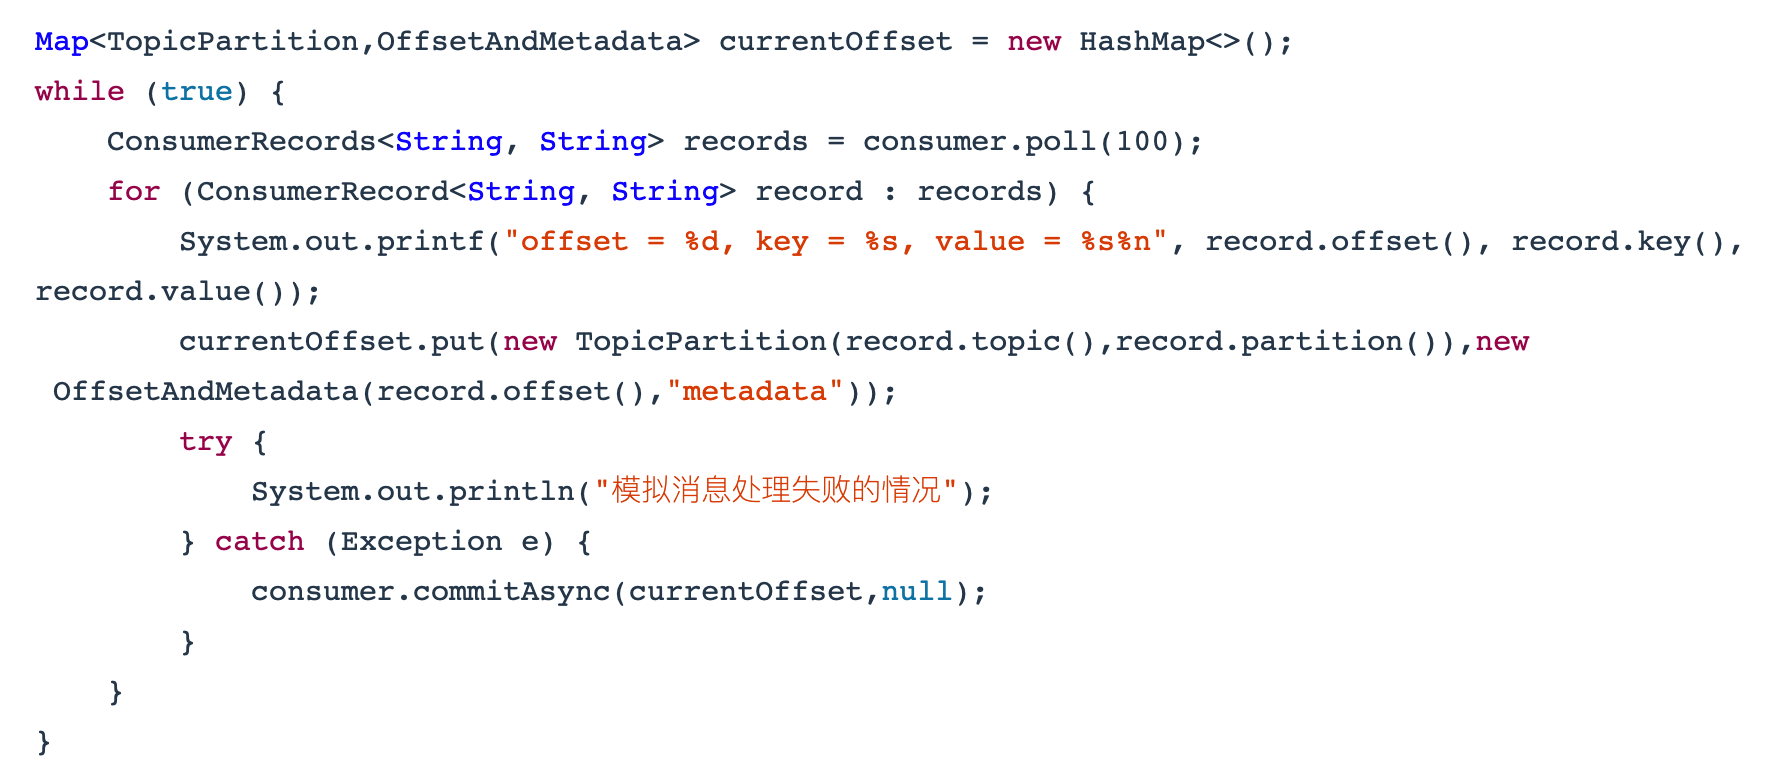
\includegraphics[width=0.9\linewidth]{image/0311}
		\caption{特定偏移量提交}
		\label{fig:0311}
	\end{figure}
	
\end{frame}
\begin{comment}
\begin{frame}[plain,t]{Kafka Consuming Model} %也可以使用\frametitle{节的名字}效果一样
	\structure{} \\  \vspace{2ex}

\end{frame}
\end{comment} 


\begin{frame}[plain,t]{Kafka Consuming Model} %也可以使用\frametitle{节的名字}效果一样
	\structure{再均衡和多线程} \\  \vspace{2ex}
	再均衡是指分区的所有权从一个消费者转移到另一个消费者的行为.
	\begin{itemize}
		\item 消费组内增删消费者
		\item 再均衡期间,消费组不可用(时间短暂)
		\item 分区重新分配到的消费者,当前状态丢失
	\end{itemize}

\vspace{2ex}
KafkaProducer是线程安全的, KafkaConsumer是非安全的.

 \vspace{2ex}
多线程消息消费最常见的方式是线程封闭,即为每个线程实例化一个KafkaConsumer对象.
	
\end{frame}
\begin{frame}[plain,t]{Kafka Consuming Model} %也可以使用\frametitle{节的名字}效果一样
	\structure{Kafka消费者重要参数配置} \\  \vspace{2ex}
\begin{itemize}
	\item fetch.min.bytes(1B)
	\item fetch.max.bytes(50MB)
	\item fetch.max.wait.ms(500ms)
	\item max.partition.fetch.bytes(1MB)
	\item max.poll.records(500条)
\end{itemize}
	
\end{frame}

\section{主题与分区}
\subsection{分区管理}
\begin{frame}[plain,t]{分区管理} %也可以使用\frametitle{节的名字}效果一样
	\structure{基本概念} \\  \vspace{2ex}
    Producer和Consumer的设计理念所针对的都是主题和分区层面的操作
    
    \vspace{2ex}
    \begin{itemize}
        \item 主题是消息的归类
        \item 分区是消息的二次归类
        \begin{itemize}
            \item 分区提供水平扩展
            \item 多副本提高数据可靠性
            \begin{itemize}
                \item 
                \item 多副本提高数据可靠性
            \end{itemize}
        \end{itemize}
    \end{itemize}


\end{frame}
\begin{frame}[plain,t]{分区管理} %也可以使用\frametitle{节的名字}效果一样
    \structure{分区管理} \\  \vspace{2ex}
    只有leader副本对外提供读写服务, follower副本只负责在内部进行消息同步.
    
    \vspace{2ex}
    针对同一个分区而言, Kafka集群中一个broker节点最多只能有一个副本.
    
    \vspace{2ex}
    Kafka集群{\color{cyan}宕机}或者添加{\color{red}新机器},可能造成负载失衡,可以通过{\color{cyan}优先副本再平衡}或者{\color{red}分区重分配}解决.
    
    
\end{frame}
\subsection{日志存储}
\begin{frame}[plain,t]{分区存储} %也可以使用\frametitle{节的名字}效果一样
    \structure{逻辑层VS物理层} \\  \vspace{2ex}
    \begin{figure}
        \centering
        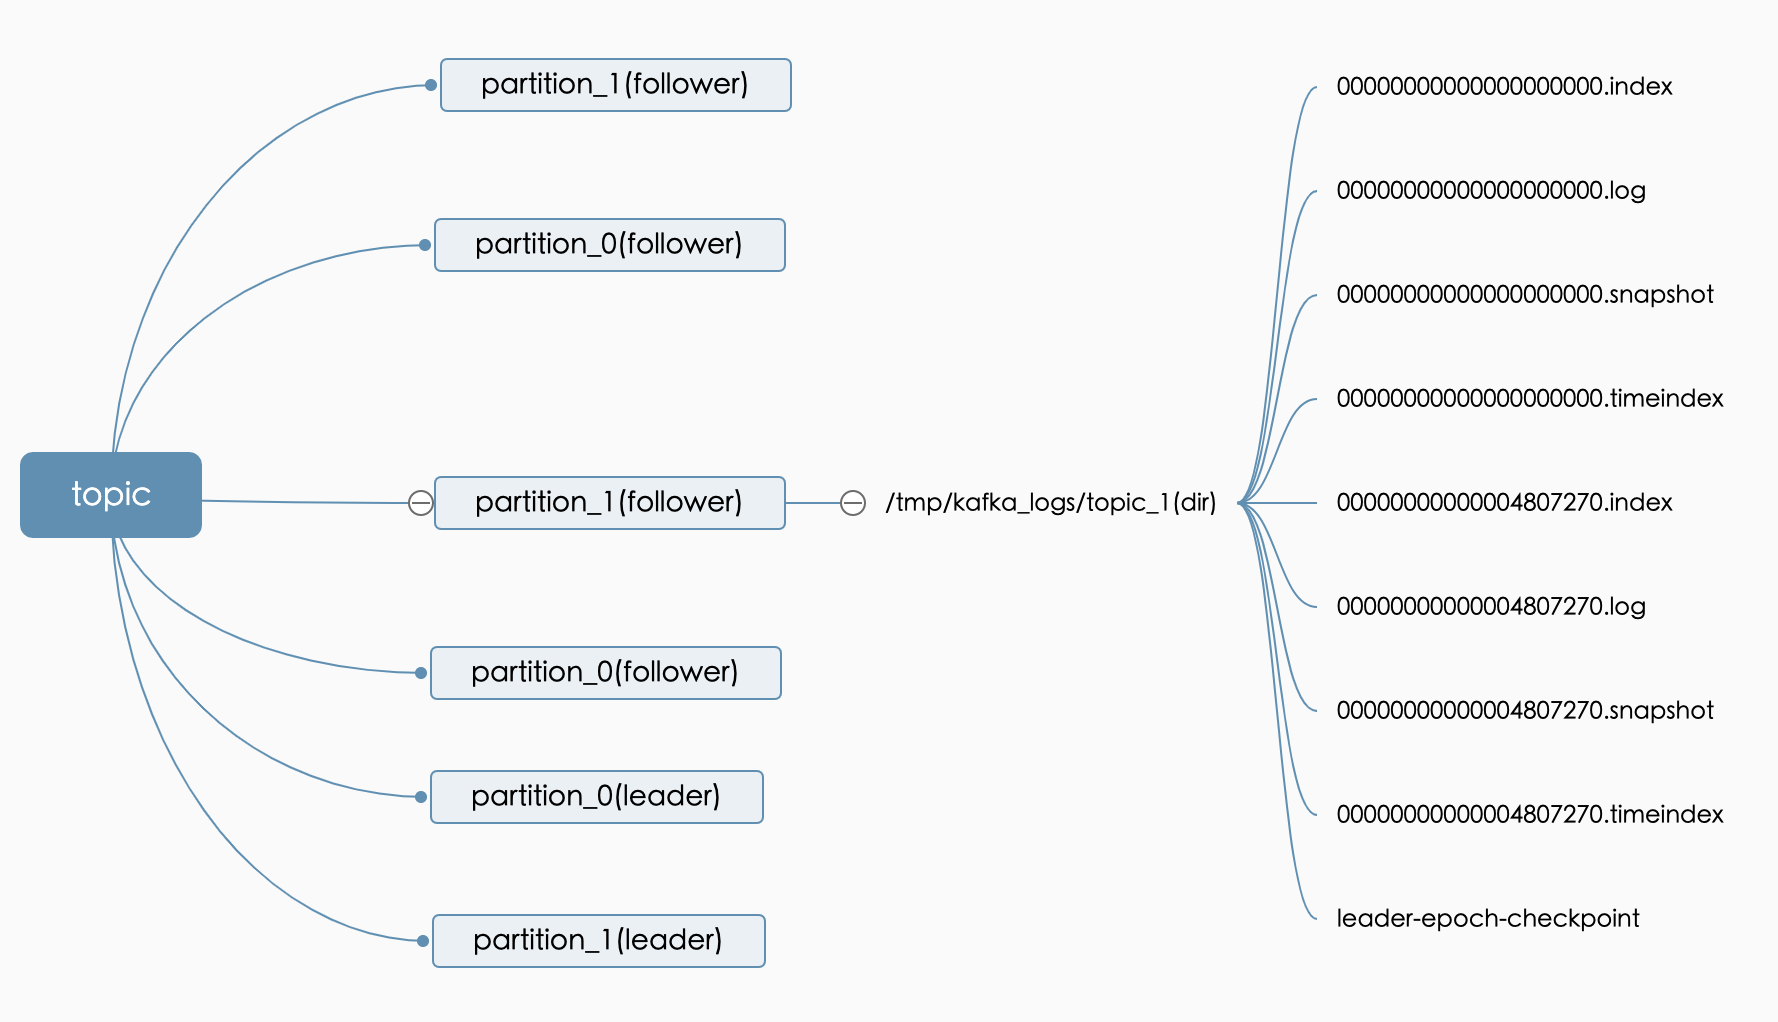
\includegraphics[width=0.9\linewidth]{image/0401.png}
        \caption{逻辑层VS物理层}
        \label{fig:0401}
    \end{figure}
    
\end{frame}





\begin{frame}[plain,t]{分区存储} %也可以使用\frametitle{节的名字}效果一样
	\structure{基准偏移} \\  \vspace{2ex}
    每个LogSegment都有一个基准偏移量baseOffset, 用来表示当前日志文件中第一条消息的offset.
    
    \vspace{2ex}
    偏移量索引文件建立了消息偏移量(offset)到物理地址的映射关系;时间戳索引文件类似.
    %偏移量是一个64位的长整数,名称固定为20位数字(不足0填充).
    
    \vspace{2ex}
    Kafka 中的索引文件是以稀疏索引(sparse index)的方式构造消息的索引. 
    %他并不保证每一个消息在索引文件中都有对应的索引项. 
    \begin{itemize}
        \item log.index.interval.bytes(默认4kb)
        \item MappedByteBuffer(Java NIO)%(将索引文件映射到内存)
    \end{itemize}
    %每当写入{\color{red}一定量(默认4KB)}的消息时, 偏移量索引文件和时间戳索引文件分别增加一个偏移量索引项和时间戳索引项.
    %通过修改 log.index.interval.bytes 的值, 改变索引项的密度.
    
\end{frame}
\begin{frame}[plain,t]{分区存储} %也可以使用\frametitle{节的名字}效果一样
    \structure{文件目录布局} \\  \vspace{2ex}
    \begin{figure}
        \centering
        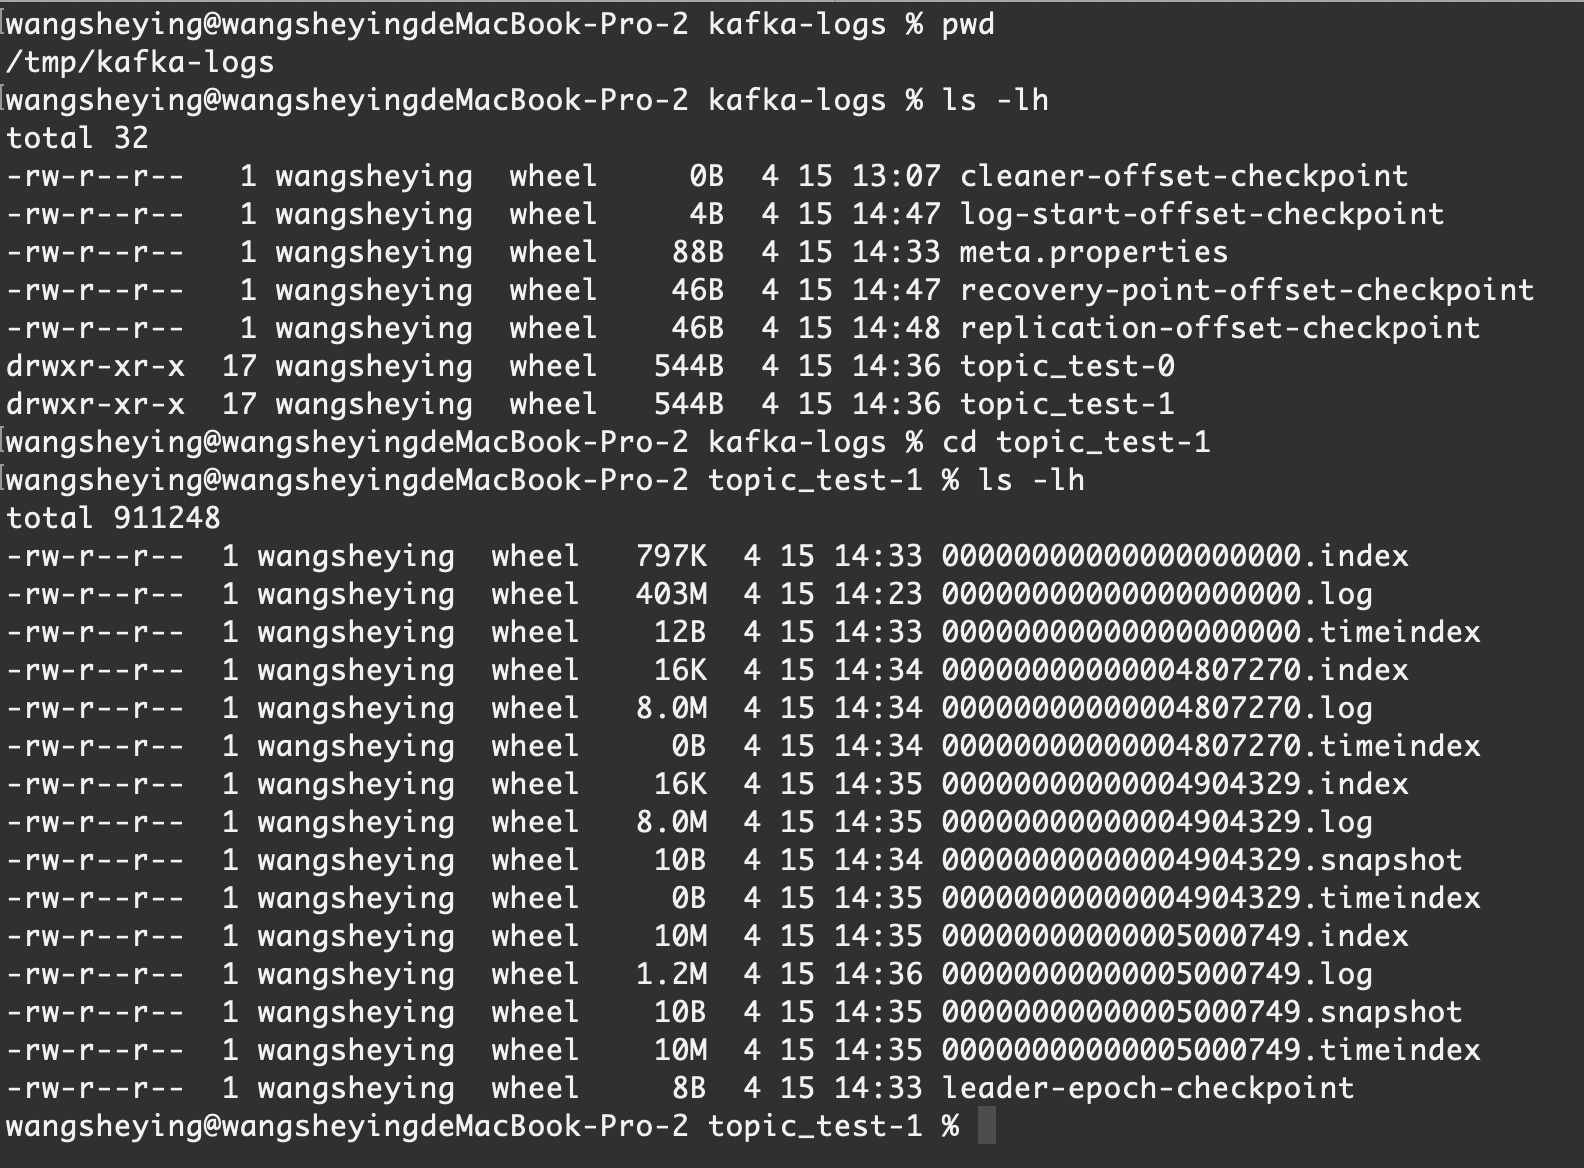
\includegraphics[width=0.8\linewidth]{image/0402.png}
        \caption{文件目录布局}
        \label{fig:0402}
    \end{figure}
    
\end{frame}
\begin{frame}[plain,t]{分区存储} %也可以使用\frametitle{节的名字}效果一样
    \structure{消息压缩} \\  \vspace{2ex}
    在一般情况下,生产者发送的压缩数据在broker中也是保持压缩状态进行存储的,
    消费者从服务端获取的也是压缩消息,消费者在处理消息之前才会解压消息,
    这样保持了端到端的压缩.
    
    \begin{itemize}
        \item gzip
        \item snappy
        \item lz4
        \item zstd
        \item uncompressed
        \item producer(默认)
    \end{itemize}
    
    
    
\end{frame}
\begin{frame}[plain,t]{分区存储} %也可以使用\frametitle{节的名字}效果一样
    \structure{V2版本消息格式(v0.11.0+)} \\  %
    \vspace{-1ex}
    \begin{figure}
        \centering
        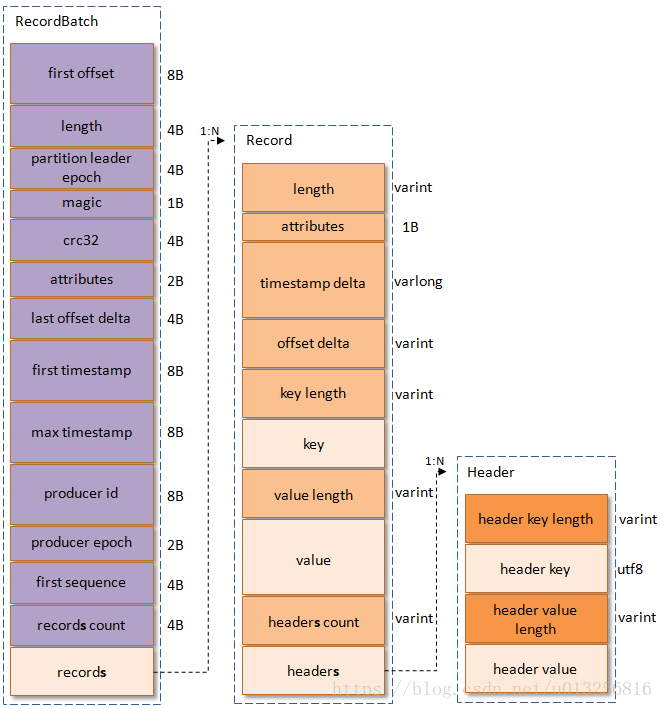
\includegraphics[width=0.65\linewidth]{image/0403}
        %\caption{V2版本消息格式}
        \label{fig:0403}
    \end{figure}
%attributes,低3位压缩类型,第4位时间戳类型,第5位是否事务中,1在,0不在
%第6位是否是控制消息,1是,0不是
    
    
    
\end{frame}
\subsection{Kafka为什么这么快}
\begin{frame}[plain,t]{Kafka为什么这么快} %也可以使用\frametitle{节的名字}效果一样
    \structure{多因素叠加} \\  \vspace{2ex}
    
    \begin{itemize}
        \item 文件分段(针对Producer,Consumer)
        \item 顺序 IO({\color{cyan}较快},针对Producer,Consumer)
        \item 日志格式(针对Producer,Consumer)
        \item page cache(主要针对Producer)%Memory Mapped Files(Java NIO)
        \item 零拷贝({\color{red}极快},仅针对Consumer) %Direct Memory Access
        \item 消除JVM GC
    \end{itemize}

%比如在producer端,FileChannel.write底层调用了pwrite,虽然pwrite系统调用会使用inode的信号量从而造成多线程竞争,但由于pwrite仅仅是写入数据到pagecache,延时非常短,所以这种争用并不是很明显——应该说这是producer实现高TPS的原因之一。另外producer端batch的设计也有助于提升TPS,因为它间接地改善了写操作模型,将部分随机写整编成顺序写;    
%而在consumer端,如果消费的数据是最近刚刚生产的,那么它们有很大概率依然在page cache中,所以Kafka源码中的FileChannel.transferTo直接调用底层sendfile实现Zero copy,将数据直接从page cache传输到socket buffer然后再通过网络传给consumer——这是consumer高TPS的原因之一。

    
\end{frame}
\begin{frame}[plain,t]{Kafka为什么这么快} %也可以使用\frametitle{节的名字}效果一样
    \structure{磁盘速度} \\  \vspace{2ex}
    As a result the performance of linear writes on a JBOD configuration with six 7200rpm SATA RAID-5 array is about 600MB/sec but the performance of random writes is only about 100k/sec—a difference of over 6000X.
    \begin{figure}
        \centering
        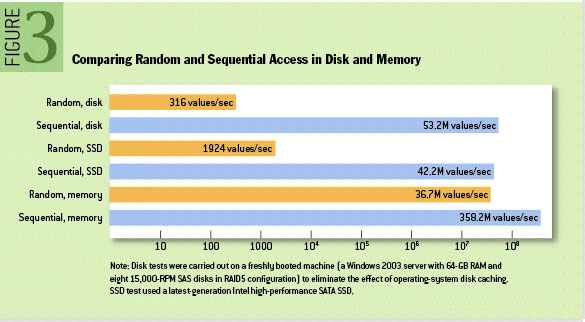
\includegraphics[width=0.7\linewidth]{image/0406}
        \caption{disk vs memory}
        \label{fig:0406}
    \end{figure}
    
    
    
\end{frame}
\begin{frame}[plain,t]{Kafka为什么这么快} %也可以使用\frametitle{节的名字}效果一样
    \structure{zero copy} \\  \vspace{2ex}
    There are 4 context switches and 2 unnecessary copies.
    
    \vspace{2ex}
    
    \begin{figure}
        \centering
        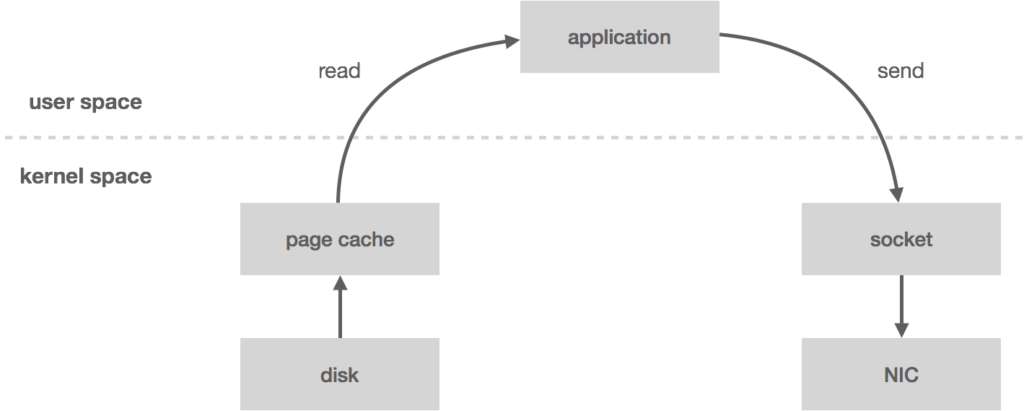
\includegraphics[width=0.9\linewidth]{image/0404}
        \caption{内核态到用户态拷贝}
        \label{fig:0404}
    \end{figure}
    
\end{frame}
\begin{frame}[plain,t]{Kafka为什么这么快} %也可以使用\frametitle{节的名字}效果一样
    \structure{zero copy} \\  %\vspace{2ex}

    
    \begin{figure}
        \centering
        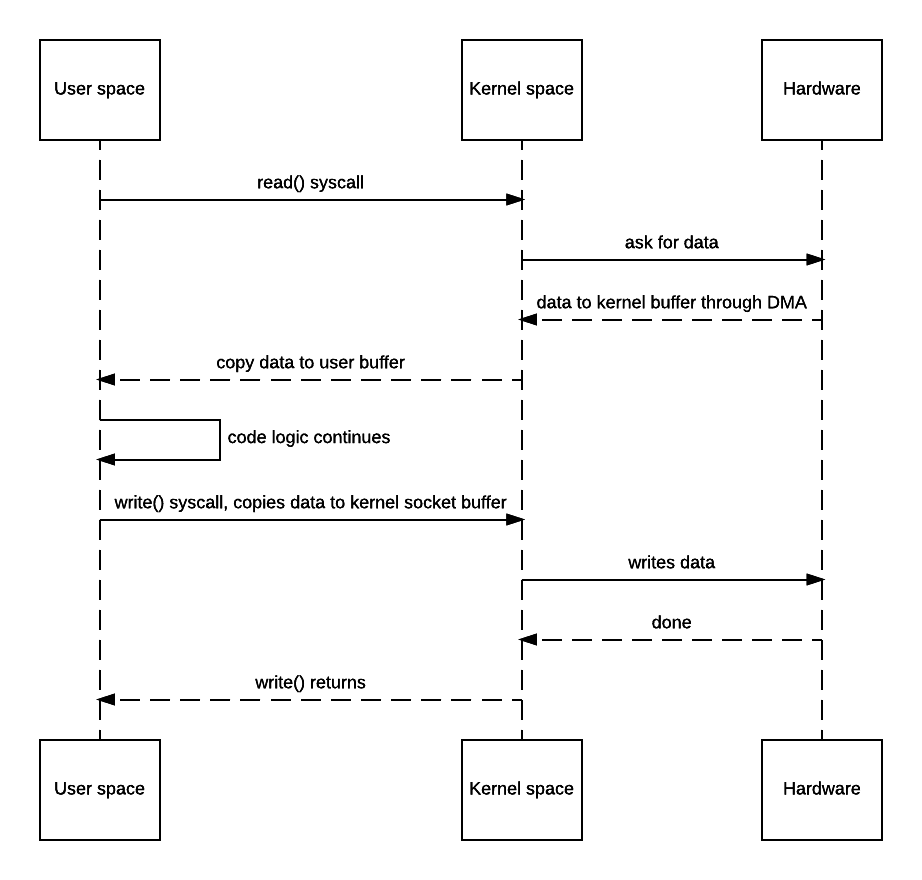
\includegraphics[width=0.7\linewidth]{image/0407}
        \caption{内核态到用户态拷贝}
        \label{fig:0407}
    \end{figure}
    
    
    
\end{frame}
\begin{frame}[plain,t]{Kafka为什么这么快} %也可以使用\frametitle{节的名字}效果一样
    \structure{zero copy} \\  \vspace{2ex}
    \begin{figure}
        \centering
        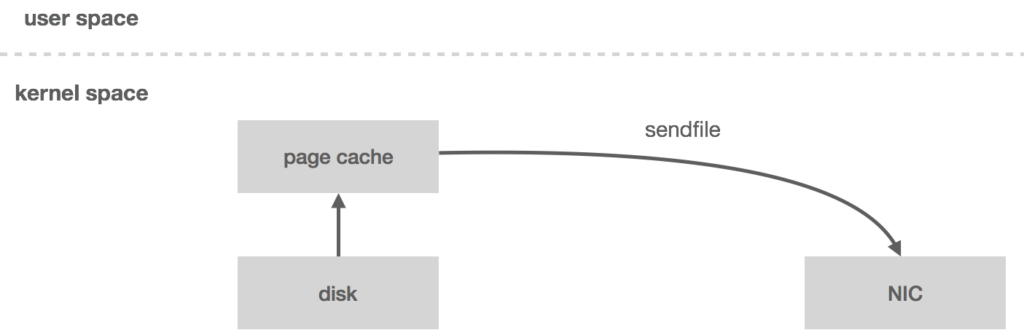
\includegraphics[width=0.9\linewidth]{image/0405}
        \caption{zero copy}
        \label{fig:0405}
    \end{figure}
    
    
\end{frame}
\begin{frame}[plain,t]{Kafka为什么这么快} %也可以使用\frametitle{节的名字}效果一样
    \structure{zero copy} \\  \vspace{2ex}
    \begin{figure}
        \centering
        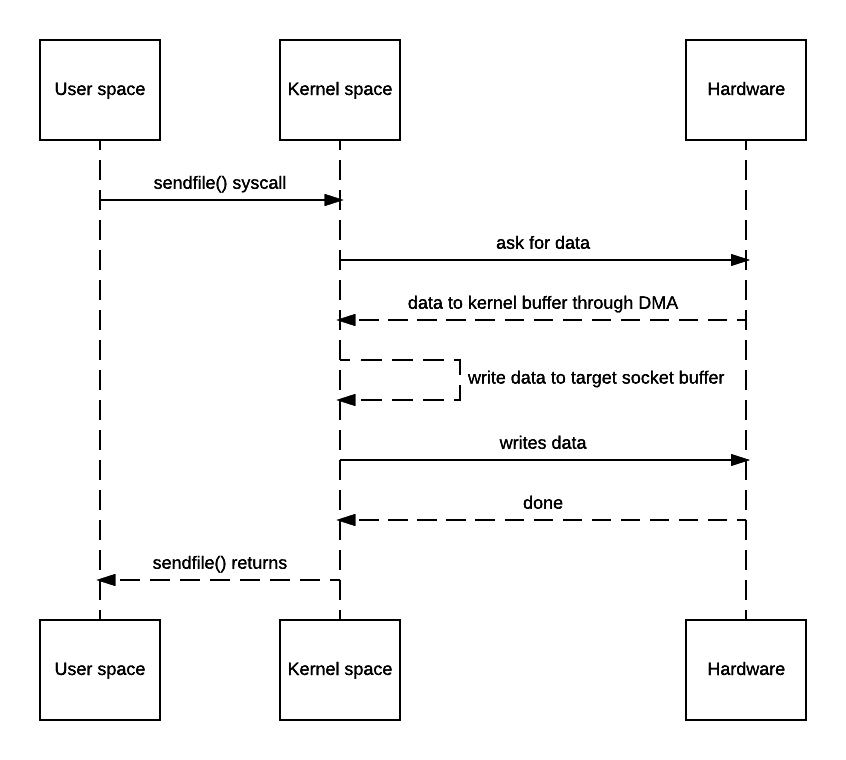
\includegraphics[width=0.7\linewidth]{image/0408}
        \caption{zero copy}
        \label{fig:0408}
    \end{figure}
    
    
\end{frame}
\begin{frame}[plain,t]{Kafka为什么这么快} %也可以使用\frametitle{节的名字}效果一样
    \structure{消除JVM GC} \\  \vspace{2ex}
    Furthermore, we are building on top of the JVM, and anyone who has spent any time with Java memory usage knows two things:
    \begin{itemize}
        \item The memory overhead of objects is very high, often doubling the size of the data stored (or worse).
        \item Java garbage collection becomes increasingly fiddly and slow as the in-heap data increases.
    \end{itemize}

\vspace{2ex}
Using the filesystem and relying on pagecache will result in a cache of up to 28-30GB on a 32GB machine without GC penalties.
    
    
    
\end{frame}


\section{深入服务端}
\subsection{协议设计}
\begin{frame}[plain,t]{协议设计} %也可以使用\frametitle{节的名字}效果一样
	\structure{基本概念} \\  \vspace{2ex}
	
\end{frame}
\begin{frame}[plain,t]{协议设计} %也可以使用\frametitle{节的名字}效果一样
    \structure{基本概念} \\  \vspace{2ex}
    
\end{frame}
\begin{frame}[plain,t]{协议设计} %也可以使用\frametitle{节的名字}效果一样
    \structure{基本概念} \\  \vspace{2ex}
    
\end{frame}
\begin{frame}[plain,t]{协议设计} %也可以使用\frametitle{节的名字}效果一样
    \structure{基本概念} \\  \vspace{2ex}
    
\end{frame}




\section{深入客户端}
\subsection{深入客户端}
\begin{frame}[plain,t]{基本概念} %也可以使用\frametitle{节的名字}效果一样
	\structure{基本概念} \\  \vspace{2ex}
	
\end{frame}

\section{可靠性探究}
\subsection{可靠性探究}
\begin{frame}[plain,t]{基本概念} %也可以使用\frametitle{节的名字}效果一样
	\structure{基本概念} \\  \vspace{2ex}
	
\end{frame}





%%=================================================================================================
\begin{frame}[plain]
	\huge
	\vfill
	\centerline{ \structure{Questions and Answers?} }
	\vfill
	
\end{frame}
\begin{frame}[plain]
	\huge
	\vfill
	\centerline{ \structure{Questions and Answers?} }
	\vfill
	\Huge
	\centerline{\alert{Thank You!} }
	\vfill
\end{frame}

%**********************************************************************************************
%                  上面就是正文,自己的内容
%        下面是标准的参考文献配置
%**********************************************************************************************
\begin{frame}[plain, t, allowframebreaks]{References}
	%  allowframebreaks,这个关键字可以使得参考文献自动断页,免得手动
	%  plain格式使得一帧的最上面是白色的,没有plain,会有色彩,可以试试
	%  t 使得正文不再是默认居中,而是在top,应该加上t,比较好看。
	\bibliographystyle{alpha}         %文献的格式apalike是[1],alpha是[Lam94]
	%\beamertemplatetextbibitems        %调整文献样式
	%\scriptsize                        %文献多时调整字体大小
	%\bibliography{math}                 %自己的文献
\end{frame}  
\end{document} 
%**********************************************************************************************
%        上面是标准的参考文献配置
%   参考文献的主题选择apalike,见《LaTeX入门》作者:刘海洋P423页(6-1-13)说明
%   apalike文献格式,按照美国心理协会(APA)的格式,提供基本的作者年代引用方式
%   避免完全不直观的数学编号可能造成的问题。这是因为beamer的文献格式比较特殊造成的
%  实例如下:
%\beamertemplatetextbibitems %该指令可使参考文献采用文字而不是图标的标注
%\begin{frame}[plain, t, allowframebreaks]{References}
%	\scriptsize
%	\bibliographystyle{apalike}
%	\bibliography{ZhangXiao-Smoothed_Analysis_of_Tensor_Decompositions} %文献命名规范,不要怕长
%\end{frame}

%**********************************************************************************************
%   学习LaTeX好的资料,有《LaTeX入门》《A Guide to LaTeX 4th Edition》 新浪微盘可下载  
%   《一份不太简短的LATEX介绍 》,网址 CTAN:/tex-archive/info/lshort 可下载  ,有中英文,每年更新
%   tex.stackexchange.com,一个美国的专业TeX问答网站,这个网站更灵活,受益匪浅
%   www.ctan.org            usepackage资料参考
%   www.texample.net       不常用,但是聚集了的专业绘图的LaTeX代码,比如画一个probability tree,
%   遇到问题,先百度Google,90%问题可解决,不行再上知乎提问,刘海洋老师,LaTeX专家,
%   可在 tex.stackexchange.com  同时提问,最基础的是读读上面的两本书,学会自己看文档
%   论文《Type setting mathematics for science and technology according to ISO 31/XI》
%   介绍排版中数学字体的选择
%***********************************************************************************************
